\subfigure[]{
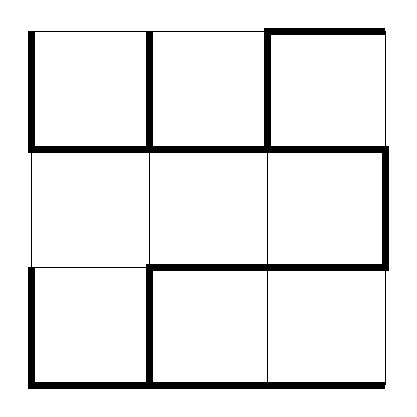
\begin{tikzpicture}
[linedecorate/.style={line width=2.5pt}]
%% set up the grid
\foreach \xstart/\xend/\y in {0/4.5/0, 0/4.5/1.5, 0/4.5/3, 0/4.5/4.5} {
  \draw (\xstart,\y) -- (\xend,\y);
  \draw (\y,\xstart) -- (\y,\xend);
}
%% draw the spanning tree
\draw[linedecorate] (0,1.5) -- (0,0) -- (4.5,0);
\draw[linedecorate] (1.5,0) -- (1.5,1.5) -- (4.5,1.5) -- (4.5,3) --
  (0,3) -- (0,4.5);
\draw[linedecorate] (1.5,3) -- (1.5,4.5);
\draw[linedecorate] (3,3) -- (3,4.5) -- (4.5,4.5);
\end{tikzpicture}
}
%%
%%
\qquad
\subfigure[]{
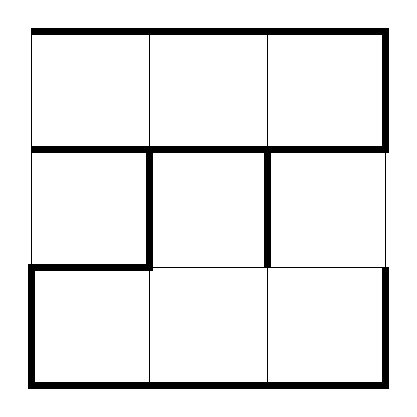
\begin{tikzpicture}
[linedecorate/.style={line width=2.5pt}]
\foreach \xstart/\xend/\y in {0/4.5/0, 0/4.5/1.5, 0/4.5/3, 0/4.5/4.5} {
  \draw (\xstart,\y) -- (\xend,\y);
  \draw (\y,\xstart) -- (\y,\xend);
}
%% draw the spanning tree
\draw[linedecorate] (4.5,1.5) -- (4.5,0) -- (0,0) -- (0,1.5) --
  (1.5,1.5) -- (1.5,3);
\draw[linedecorate] (0,4.5) -- (4.5,4.5) -- (4.5,3) -- (0,3);
\draw[linedecorate] (3,1.5) -- (3,3);
\end{tikzpicture}
}
